\section{Introduction}

Robotic manipulation of deformable objects tends to be challenging due to high-dimensional, 
continuous state-action spaces and due to the complicated dynamics of
deformable objects.

Despite these challenges, recent
work~\cite{Schulmanetal_IROS2013, Schulmanetal_ISRR2013} has shown
promising results in enabling robotic manipulation of deformable
objects through learning from demonstrations. This work
uses non-rigid registration to register a training scene onto the
current test scene, and then extrapolates this registration to perform
\emph{trajectory transfer} of the robot gripper trajectory.  The
effectiveness of this approach was validated through experiments in
knot-tying and suturing.

For complex tasks, often demonstrations correspond to steps in the task, rather
than the entire task itself. Figure~\ref{fig:knot_steps} shows an example
of the steps involved in tying an overhand knot.
In general, a single demonstration for a step in the task cannot be expected
to cover all possible scenarios that arise during execution.
The natural solution to this is to use a library of demonstrations with
multiple demonstrations for each step.

Realizing these benefits requires a robust technique to select a good trajectory to
transfer.  Certain trajectories will generalize better than others, and particular sequences of 
demonstrations may perform tasks more efficiently than others.
%The existence of poor or brittle demonstrations can very negatively 
%affect performance.
%For example, a demonstration in knot tying that involves a grasp
%unnecessarily close to the edge of the rope may generalize poorly
%to new scenes, compared to other more robust demonstrations of the task.

The original paper presenting the approach of trajectory transfer
prescribes choosing the trajectory segment from the demonstrations
library with the lowest warping cost onto the current scene~\cite{Schulmanetal_ISRR2013}.
This approach does not account for the inherent generalizability
of a particular demonstration. For brittle demonstrations (e.g. grabbing
near the edge of a rope), a small change in the rope can have low registration
cost, but the transferred trajectory will fail.
As a result, such an approach may fail to accomplish tasks
that would be possible with a different sequence of trajectories.

\begin{figure}[t]
  \centering
    \noindent
    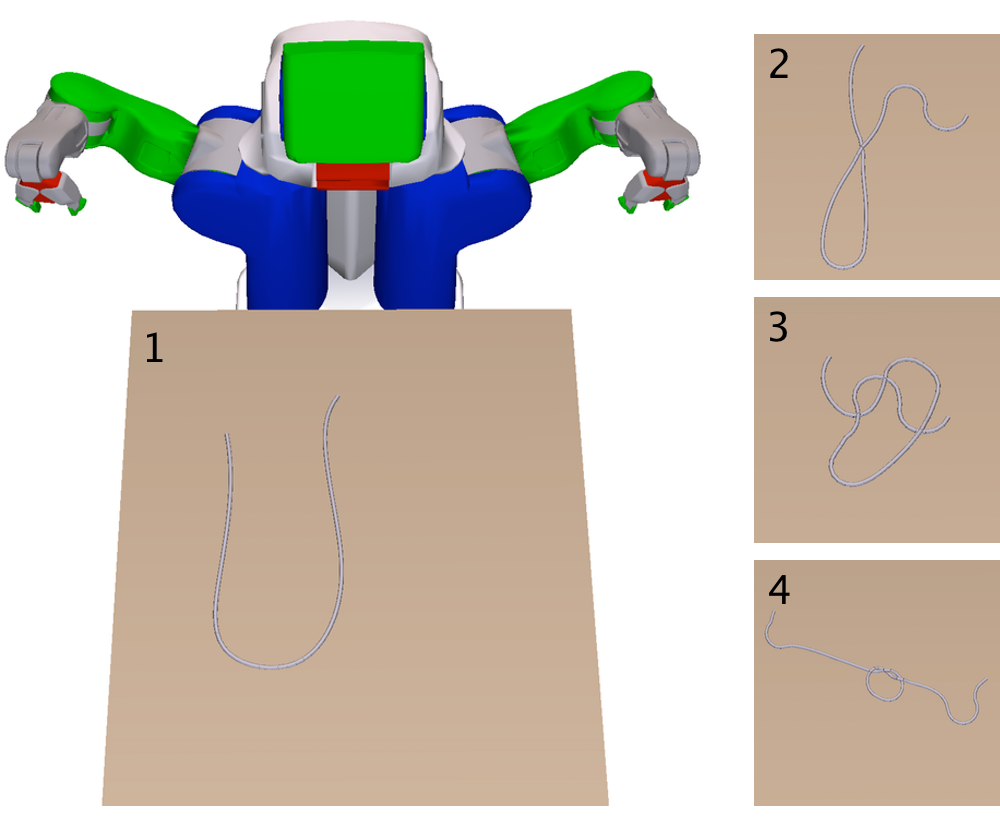
\includegraphics[width=0.45\textwidth]{figures/knot_steps_num.png}
  \caption{The overhand knot manipulation task in our benchmark.
           A standard knot tie takes three steps, as shown in this
           particular execution from our benchmark.}
  \label{fig:knot_steps}
\end{figure}

%TODO: make into list; link to sections/subsections in the paper
In this paper, we present a solution to the demonstration selection problem that
can account for the variability in robustness of demonstrations and incorporates the
sequential nature of our tasks. Our contributions are as follows:
(i) We formulate the demonstration selection problem as a Markov Decision
Process (MDP); (ii) We present Max-Margin Q-Learning (\mmql{}), a method for
approximating Q-functions from expert-guided task executions, based on the optimality
of the expert's action selection; (iii) We describe task-independent
features that are rich enough to allow learning but make no additional
assumptions beyond those of trajectory transfer; and (iv) We develop an unsupervised
labeling method that we call Leave-One-Out Labeling (LOOL) that allows
us to apply \mmql{} with no human input beyond providing a library of demonstrations.

We developed a knot-tying benchmark for evaluating the effectiveness of
our proposed approach.   This benchmark is available at
\href{https://sites.google.com/site/rss2014mmql}{sites.google.com/site/rss2014mmql}). The
nearest neighbor approach described in \citet{Schulmanetal_ISRR2013} achieves a
68.8\% success rate on this benchmark.  The greedy policy with respect to our learned
approximate Q-function achieves a success rate of 85.6\%. Augmenting our
policy with a simulator and beam search raises the success rate to 95.2\%.
%The best possible success rate with our demonstration library is 95.2\%.

While our running example and experiments deal with knot tying, our presented
\mmql{} approach makes no assumptions about the
specifics of the task except for the availability of point clouds of
the scene.
